\section{Zielsetzung}

In diesem Versuch sollen Beugungsbilder von zwei Einzelspalten untersucht werden, um auf die Größe dieser rückschließen zu können.
Analog soll die Breite und der Abstand eines Doppelspaltes bestimmt werden.


\section{Theorie}
\label{sec:Theorie}

Wenn die Abmessungen einer Blende in der Größenordnung der Wellenlänge $\lambda$ des Lichtes sind, so können Beugungsbilder beobachtet werden.
Es wird dabei zwischen der Fresnel'schen Beugung und der Fraunhofer Näherung unterschieden.
Bei ersterer werden Lichtstrahlen betrachtet, die nah an der Blende aufeinander treffen, also unter verschiedenem Winkel $\Phi$ abgelenkt werden.
In diesem Versuch wird jedoch die Fraunhofer Näherung betrachtet, bei welcher die Distanz zwischen Blende und Schirm beziehungsweise Detektor sehr groß gegen die Blendengröße gewählt wird,
sodass die interferierenden Strahlen als parallel angenommen werden können. Diese Schema ist in \autoref{fig:fraunhofer-schematisch} zu finden.

\begin{figure}
    \centering
    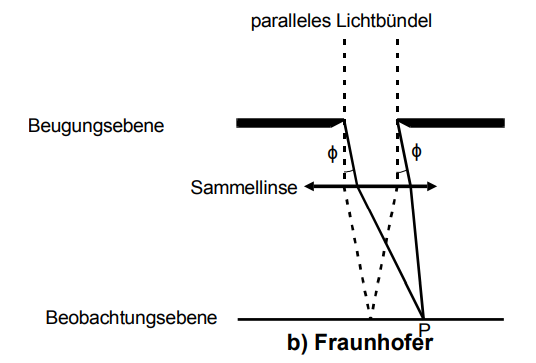
\includegraphics[width=0.9\textwidth]{content/fraunhofer-schematisch.png}
    \caption{Veranschaulichung der Fraunhofer Beugung am Einzelspalt \cite{V406}.}
    \label{fig:fraunhofer-schematisch}
\end{figure}

Die Beugung selbst kann mit dem Huygen'schem Prinzip erklärt werden.
Bei diesem wird angenommen, dass sich an jedem Punkt einer Welle eine neue kugelförmige Elementarwelle ausbreitet.
Diese interferieren miteinander und bilden so neue Wellenfronten.
An dem Spalt selbst breiten sich diese dann nicht nur in die eigentliche Laufrichtung aus, sondern auch seitlich.
Insgesamt muss über jedes einzelne Strahlenbündel summiert werden, um die Amplitude unter einem Winkel $\Phi$ zu bestimmen.
Aufgrund der geringen Größe jener, geht die Summation in eine Integration der gesamten Spaltbreite $b$ über.
im Allgemeinen werden Wellen durch die Gleichung

\begin{equation}
    \label{eqn:wellengleichung}
    A(z,t) = A_0 \text{exp} \bigg( i \bigg( \omega t - \frac{2\pi z}{\lambda} \bigg) \bigg)
\end{equation}

beschrieben. Dabei ist $\omega$ die Kreisfrequenz und $A_0$ die Amplitude.
Werden zwei Strahlen, wie in \autoref{fig:phasenunterschied} zu sehen, an zwei verschiedenen Orten mit Abstand $x$ unter gleichem Winkel $\Phi$ ausgesendet, so kann ein Phasenunterschied

\begin{equation}
    \label{eqn:phasenunterschied}
    \delta = \frac{2 \pi \sin (\Phi)}{\lambda}
\end{equation}

festgestellt werden.

\begin{figure}
    \centering
    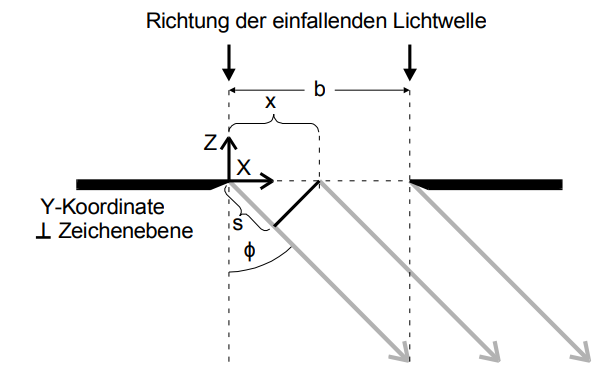
\includegraphics[width=0.9\textwidth]{content/phasenunterschied.png}
    \caption{Schematische Skizze zum Gangunterschied zweier Lichtstrahlen \cite{V406}.}
    \label{fig:phasenunterschied}
\end{figure}

Nach der Integration und Umformungen ergibt sich für die Amplitude für einen Winkel $\Phi$ folgende Beziehung:

\begin{equation}
    \label{eqn:amp-integration}
    B(z, t, \Phi) = A_0 \text{exp} \bigg( i \bigg( \omega t - \frac{2 \pi z}{\lambda} \bigg) \bigg) \cdot \text{exp} \bigg( \frac{i \pi b \sin (\Phi)}{\lambda} \bigg) \cdot \frac{\lambda}{\pi \sin( \Phi )} \sin \bigg( \frac{\pi b \sin(\Phi )}{\lambda} \bigg).
\end{equation}

Die beiden exponentiellen Terme beschreiben dabei eine Phase. Für die experimentelle Untersuchung sind die letzten beiden Terme relevant.

Aufgrund der hohen Frequenz von Licht ist es schwierig die Amplitude zu messen, weshalb hier die zeitlich gemittelte Intensität $I$ betrachtet wird. Dabei gilt die Relation

\begin{equation}
    \label{eqn:intensitaet-einzel}
    I ( \Phi ) \prop B^2 ( \Phi ) = A_0^2 b^2 \bigg( \frac{\lambda}{\pi b \sin ( \Phi )} \bigg)^2 \cdot \sin^2 \bigg( \frac{\pi b \sin(\Phi)}{\lambda} \bigg)^2.
\end{equation}

Analog kann der Doppelspalt als Überlagerung von zwei Einzelspalten betrachtet werden.
Dabei ergibt sich für die Intensitätsverteilung

\begin{equation}
    \label{eqn:intensitaet-doppel}
    I ( \Phi ) \prop B^2 (\Phi ) = 4 \cos^2 \bigg ( \frac{\pi s \sin( \Phi )}{\lambda} \bigg)^2 \cdot \bigg( \frac{\lambda}{\pi b \sin( \Phi )} \bigg)^2 \cdot \sin^2 \bigg( \frac{\pi b \sin ( \Phi )}{\lambda} \bigg),
\end{equation}

wobei $b$ die Breite der Einzelspalte und $s$ deren Abstand ist.